% Results
% Every number comes from reports/results.csv, reports/results_table.md, notebooks/02_evaluation.ipynb
% or reports/checks.

\section{Results}

All models are scored on the same 6\,727\,699 labelled test pixels (1\,689 patches); 1.25\% of them burn on
day $t+1$, about one pixel in 80. Precision, recall and F1 use the threshold that maximises F1 on the eval split;
PR AUC, ROC AUC and recall at a fixed false positive rate (FPR) need no threshold.

\subsection{Overall performance}

\begin{table*}[t]
\centering
\caption{Test results. Precision (P), recall (R) and F1 at the threshold chosen on the eval split. Bold: best per
column. PR AUC reported by Huot et al.~\cite{huot2022} for their models is in Table~\ref{tab:relwork}.}
\label{tab:results}
\begin{tabular}{lccccccc}
\hline
Model & PR AUC & ROC AUC & P & R & F1 & R @ 1\% FPR & R @ 5\% FPR \\
\hline
Persistence & 0.106 & 0.633 & 0.357 & 0.273 & 0.309 & 0.273 & 0.273 \\
Logistic regression (raw) & 0.146 & 0.798 & \textbf{0.378} & 0.266 & 0.312 & 0.281 & 0.319 \\
Random forest (raw) & 0.157 & 0.816 & 0.371 & 0.270 & 0.312 & 0.279 & 0.362 \\
XGBoost (raw) & 0.145 & 0.795 & 0.337 & 0.257 & 0.292 & 0.267 & 0.375 \\
XGBoost (tuned, 35 features) & \textbf{0.257} & \textbf{0.906} & 0.242 & \textbf{0.526} & \textbf{0.332} & \textbf{0.388} & \textbf{0.675} \\
LightGBM (tuned, 35 features) & 0.248 & 0.903 & 0.242 & 0.520 & 0.331 & 0.384 & 0.671 \\
\hline
\end{tabular}
\end{table*}

\begin{figure*}[!t]
\centering
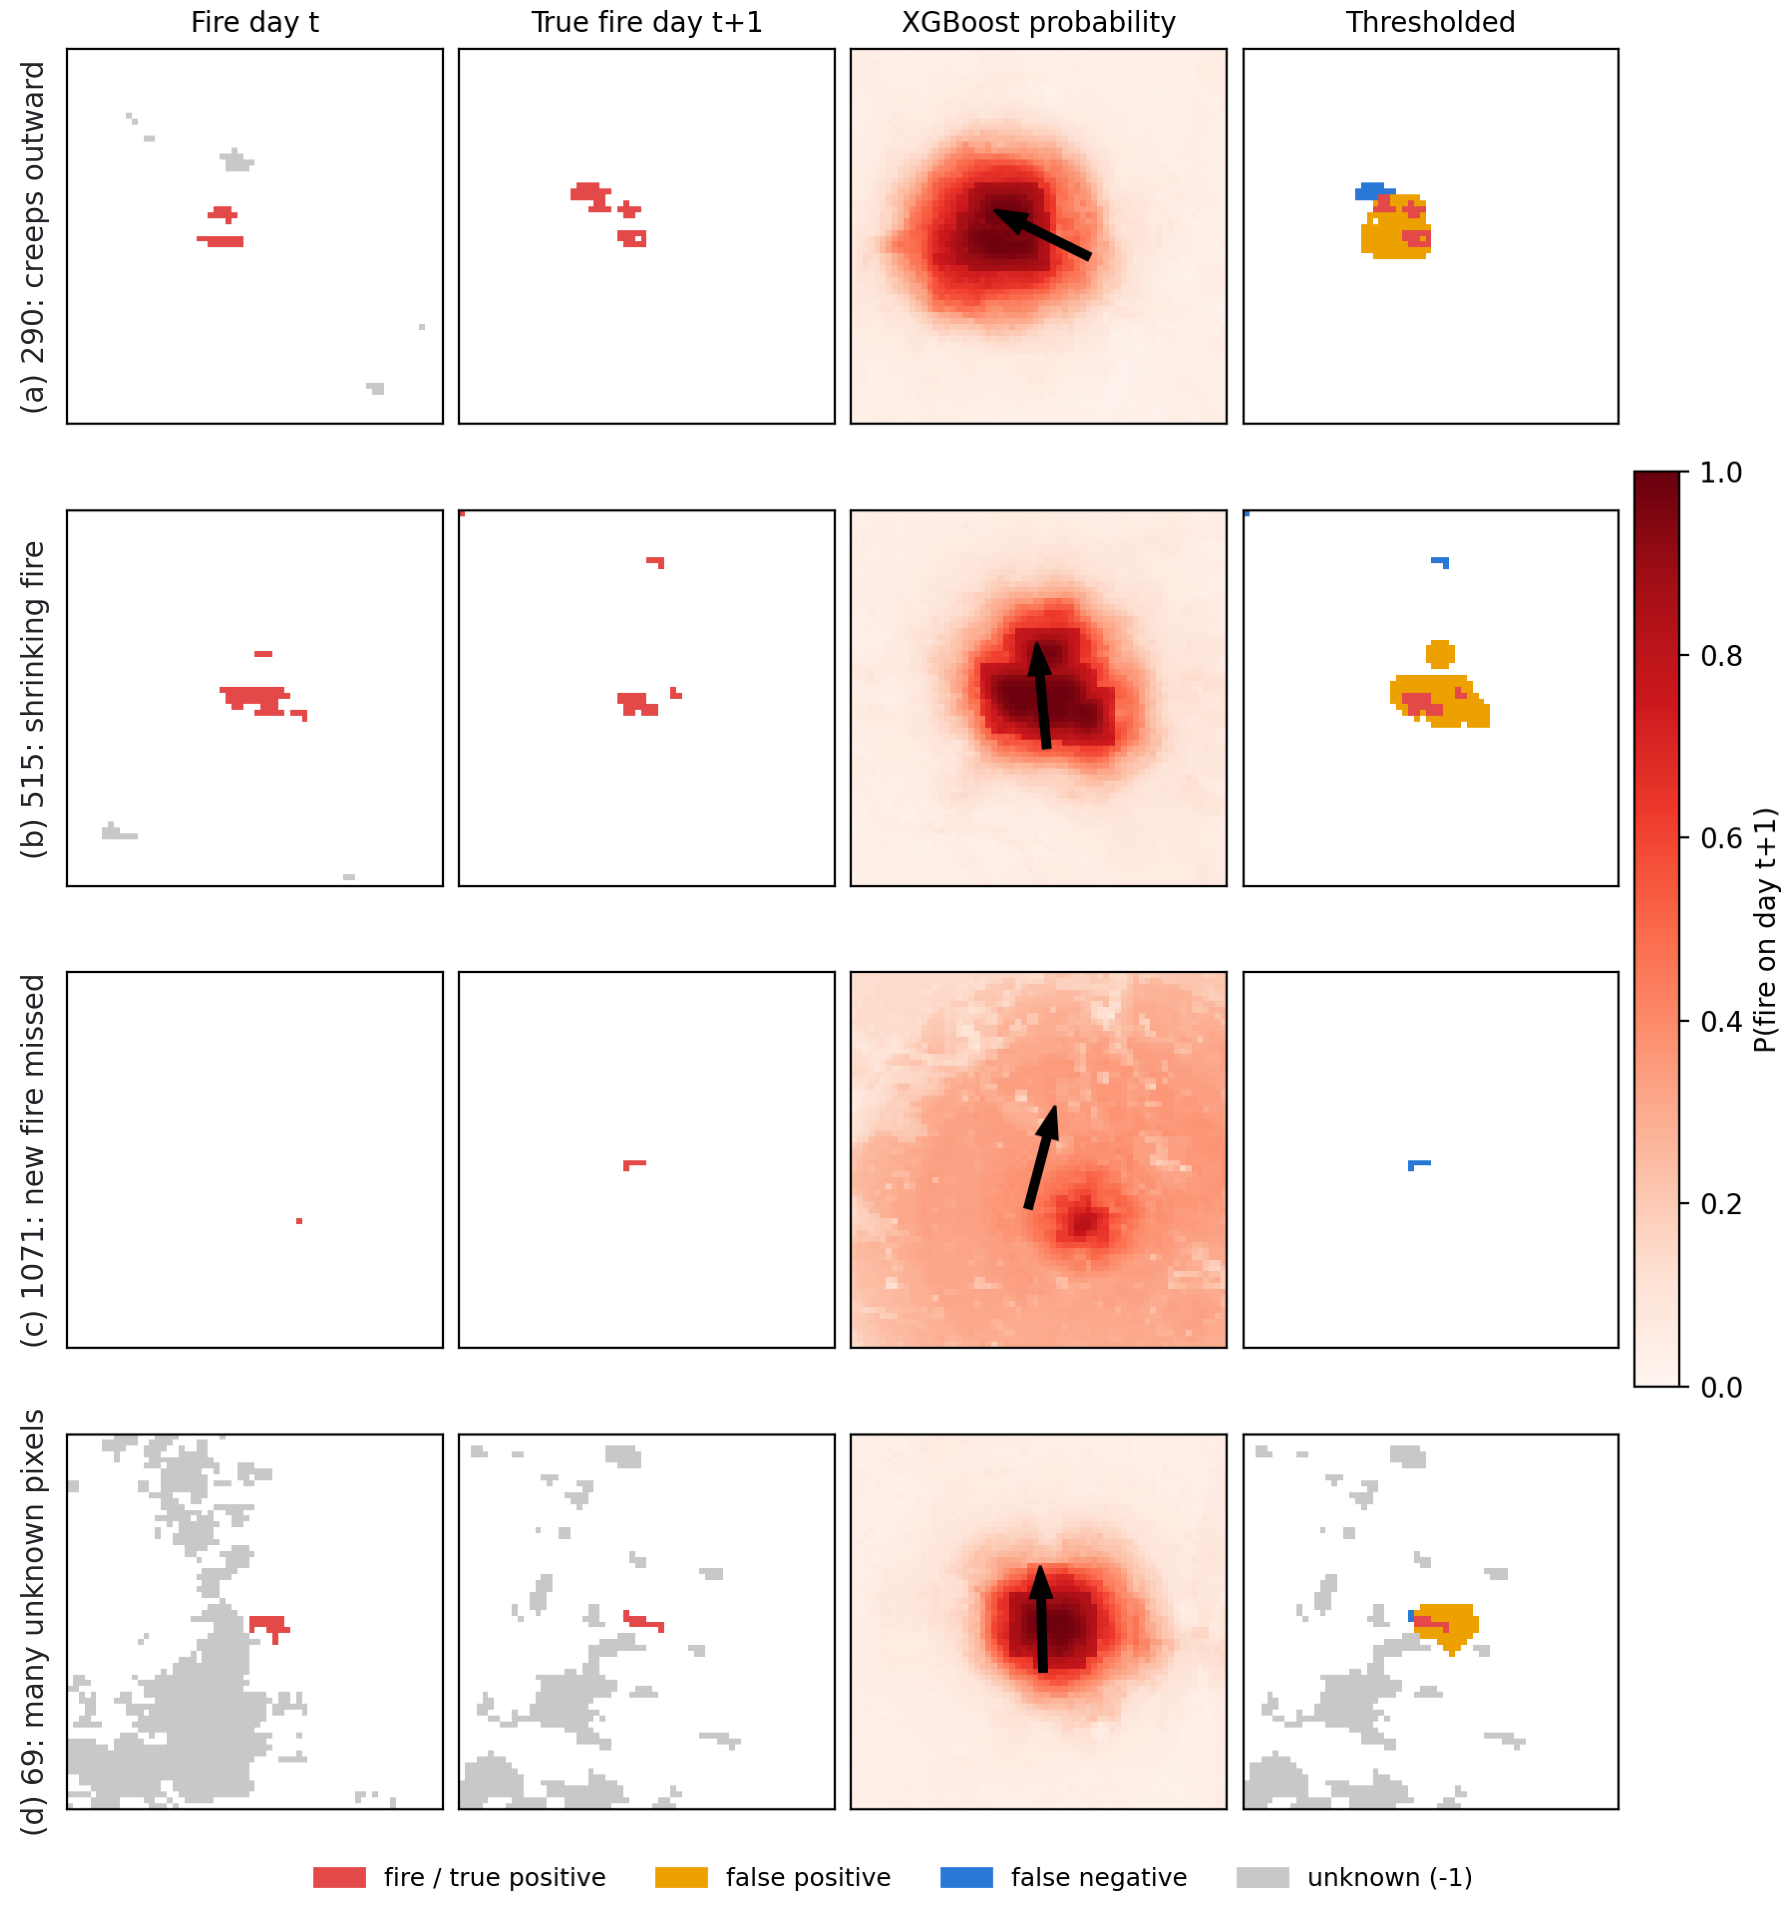
\includegraphics[width=0.72\textwidth]{figures/eval_prob_maps_selected.png}
\caption{Tuned XGBoost on four test patches that show its typical behaviour (all ten random patches are in
Fig.~\ref{fig:maps_all}). Columns: fire on day $t$, true fire on day $t+1$, predicted probability (arrow: direction the
wind blows to), and prediction at the eval threshold. Drawn from the rebuilt model (Appendix~\ref{app:checks}).}
\label{fig:maps}
\end{figure*}

The tuned XGBoost is the best model on every threshold-free metric (Table~\ref{tab:results}): PR AUC 0.257 against
0.145--0.157 for the raw-channel models and 0.106 for persistence. LightGBM is close behind (0.248), so the features
matter far more than the boosting library; the ablation (Table~\ref{tab:ablation}) traces the gain to the
fire-neighbourhood group. At the eval threshold the tuned models find 52--53\% of next-day fire at 24\% precision,
about twice the recall of the baselines (26--27\%), and reach the best F1 (0.332); a threshold tuned on test would give
only 0.358, so the eval threshold transfers well. Our persistence (0.106) is close to the paper's (0.115); the tuned
XGBoost is above their neighbour-feature random forest (0.225) but below their CNN (0.284). Both values lie inside our
95\% bootstrap interval over fire events (0.188-0.325, Appendix~\ref{app:checks}), so neither difference is significant
on test-sampling grounds. The same check shows that the gap to LightGBM is small but consistent (0.007, higher in 99\%
of paired resamples), and the gain over the raw-channel models clear (0.10, interval 0.09-0.12).

\begin{figure}[t]
\centering
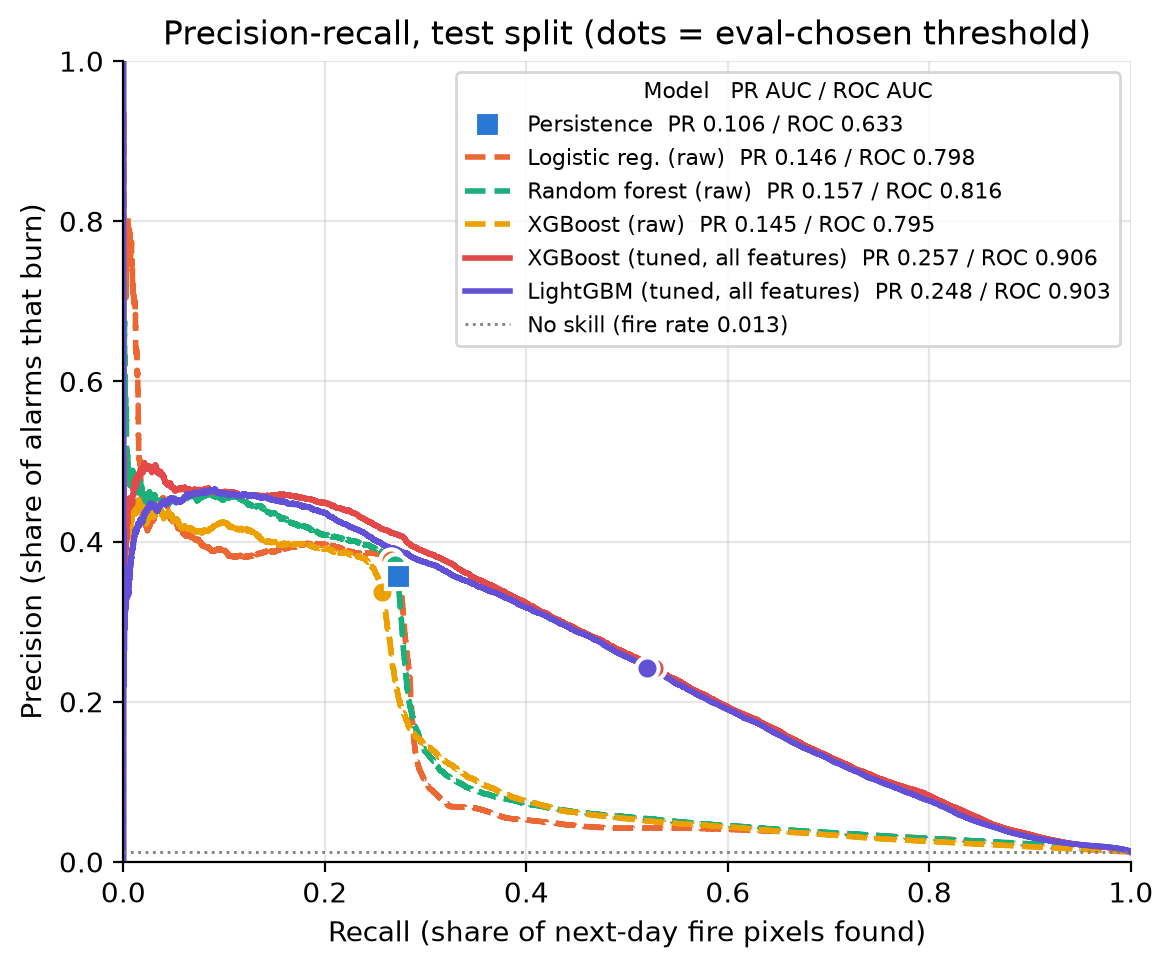
\includegraphics[width=\columnwidth]{figures/eval_pr_curves.png}
\caption{Precision--recall curves on the test split. Dots: operating point at the eval-chosen threshold.
Persistence outputs only 0 or 1, so it is a single point.}
\label{fig:pr}
\end{figure}

The tuned models stay above every baseline along the whole PR curve (Fig.~\ref{fig:pr}). The raw-channel models rank
already-burning pixels first and have little signal for new fire, so their operating points sit on top of persistence.
ROC AUC is 0.795--0.906 for every learned model while PR AUC stays at or below 0.257; Section~\ref{sec:theory_pr}
explains why PR AUC is the more informative metric at this prevalence.

\subsection{Probability maps}

The predicted probability is a smooth halo around the day-$t$ fire (Fig.~\ref{fig:maps}), following its shape and
stretched slightly toward where the wind blows (Fig.~\ref{fig:maps}d; patch 33 in Fig.~\ref{fig:maps_all}). After
thresholding, the prediction is roughly the day-$t$ fire grown by a few kilometres. It catches fire that stays or creeps
outward (Fig.~\ref{fig:maps}a; also patches 856 and 1432), paints a false-positive ring around small fires that shrink
(Fig.~\ref{fig:maps}b, patch 515: 48 to 29 burning pixels, 114 false positives), and misses fire that appears away from
the day-$t$ fire (Fig.~\ref{fig:maps}c): in patches 120, 443, 1071 and 1369 not one next-day fire pixel is found.
Unknown pixels (grey) are left out of every metric. The raw scores are shifted by the 5:1 subsampled table and the class
weighting, which is why the eval threshold is as high as 0.915; undoing that shift in closed form gives probabilities
close to the observed fire rate (Section~\ref{sec:theory_imb}). Only the ranking and the threshold affect the metrics.

\subsection{Interpretability and physical plausibility}

\begin{figure}[t]
\centering
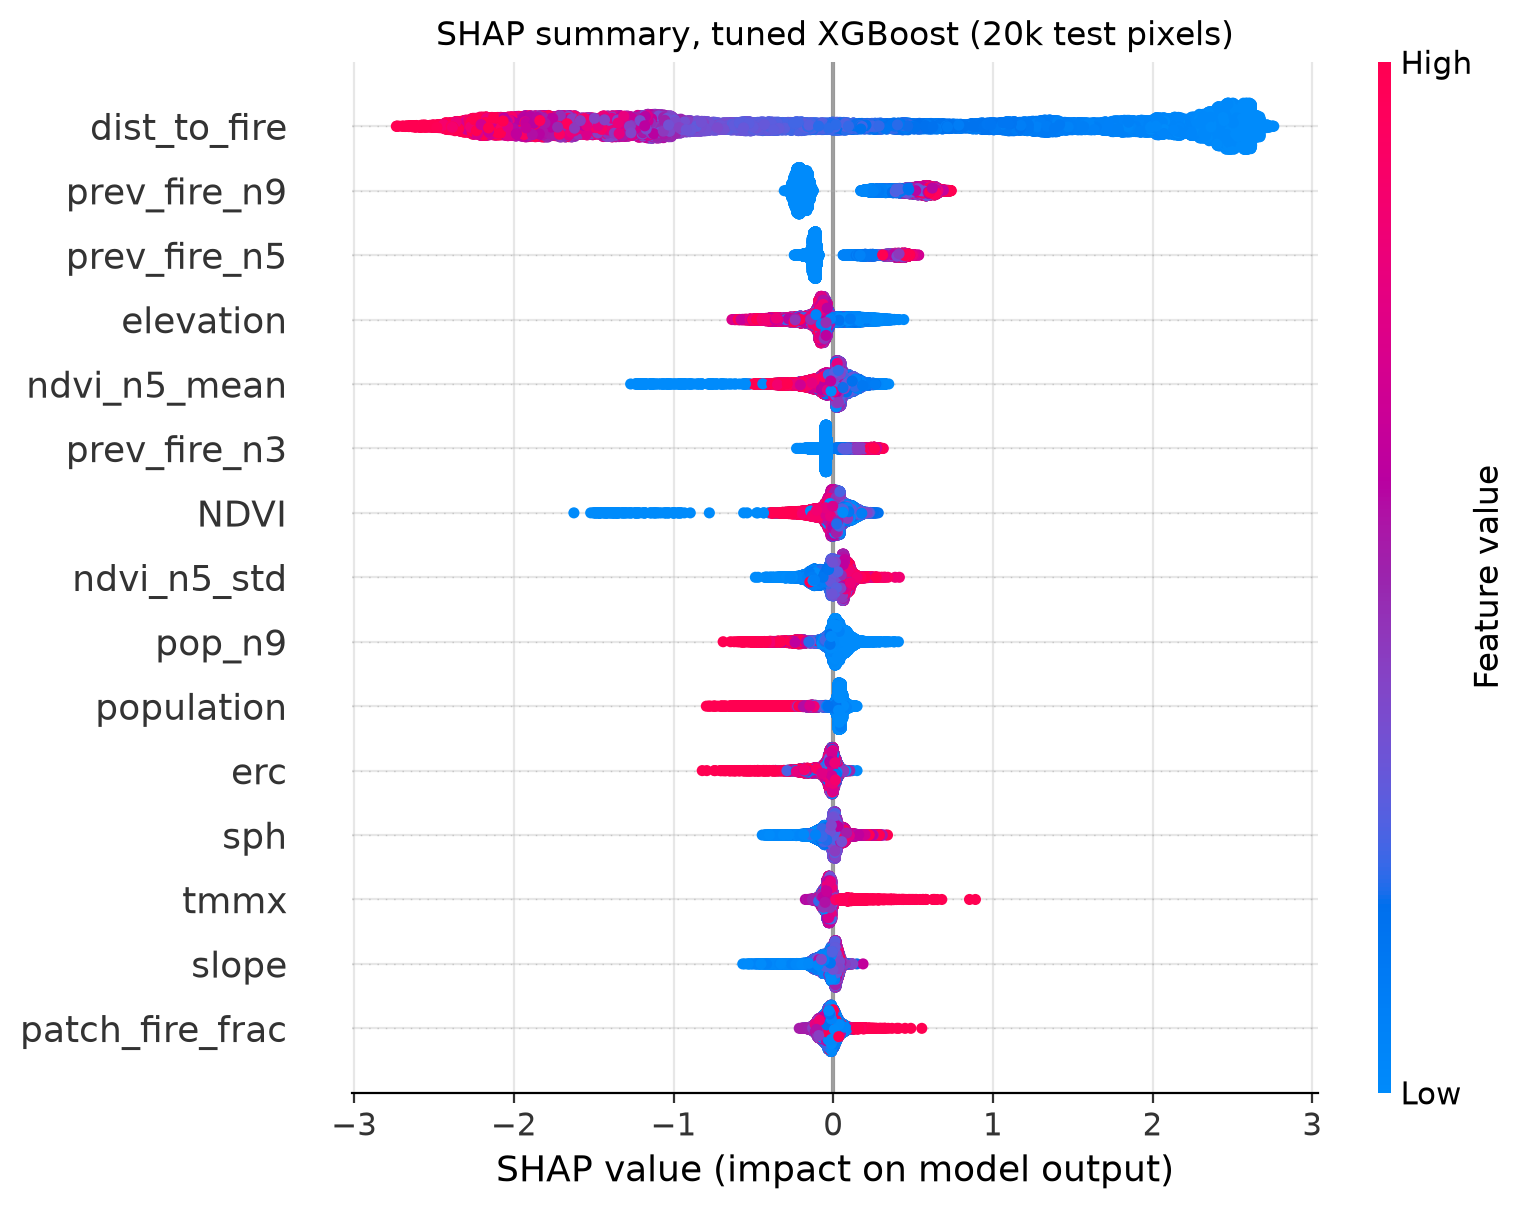
\includegraphics[width=\columnwidth]{figures/eval_shap_summary.png}
\caption{SHAP values of the tuned XGBoost on 20\,000 test pixels (10\,000 fire, 10\,000 no fire). Positive values push
the prediction toward fire; colour shows the feature value.}
\label{fig:shap}
\end{figure}

SHAP values~\cite{lundberg2017}, computed with TreeSHAP~\cite{lundberg2020}, of the refitted model (identical predictions, Fig.~\ref{fig:shap}) confirm the gain ranking in the Feature
Engineering section: the fire-neighbourhood group contributes 2.29 log-odds on average, against 0.40 for weather, 0.22
for vegetation, 0.20 for terrain and 0.13 for human features. Most effects have the expected sign (Spearman $\rho$
between feature value and SHAP value):
pixels closer to fire and with more fire nearby get higher risk (\texttt{dist\_to\_fire} $-0.97$,
\texttt{prev\_fire\_n3} $+0.75$); drier air raises it
(\texttt{vpd} $+0.72$, \texttt{min\_rel\_humidity} $-0.64$); and so do stronger wind (\texttt{vs} $+0.72$) and fire
upwind (\texttt{upwind\_fire\_k2/k4/k8} $+0.69/+0.61/+0.49$, \texttt{fire\_wind\_alignment} $+0.91$). NDVI is
mixed: bare ground and water (lowest NDVI, no fuel) get the most negative SHAP values, while over the main range greener,
moister vegetation lowers risk ($\rho=-0.82$). One sign is not physical: high ERC (dry fuel) lowers the prediction ($\rho=-0.13$ overall, with the strongest negative SHAP values
at the highest ERC). ERC is a coarse regional value, almost constant over a patch, so the model most likely uses it as a
proxy for where and when a fire is, not as a cause.

\begin{figure}[t]
\centering
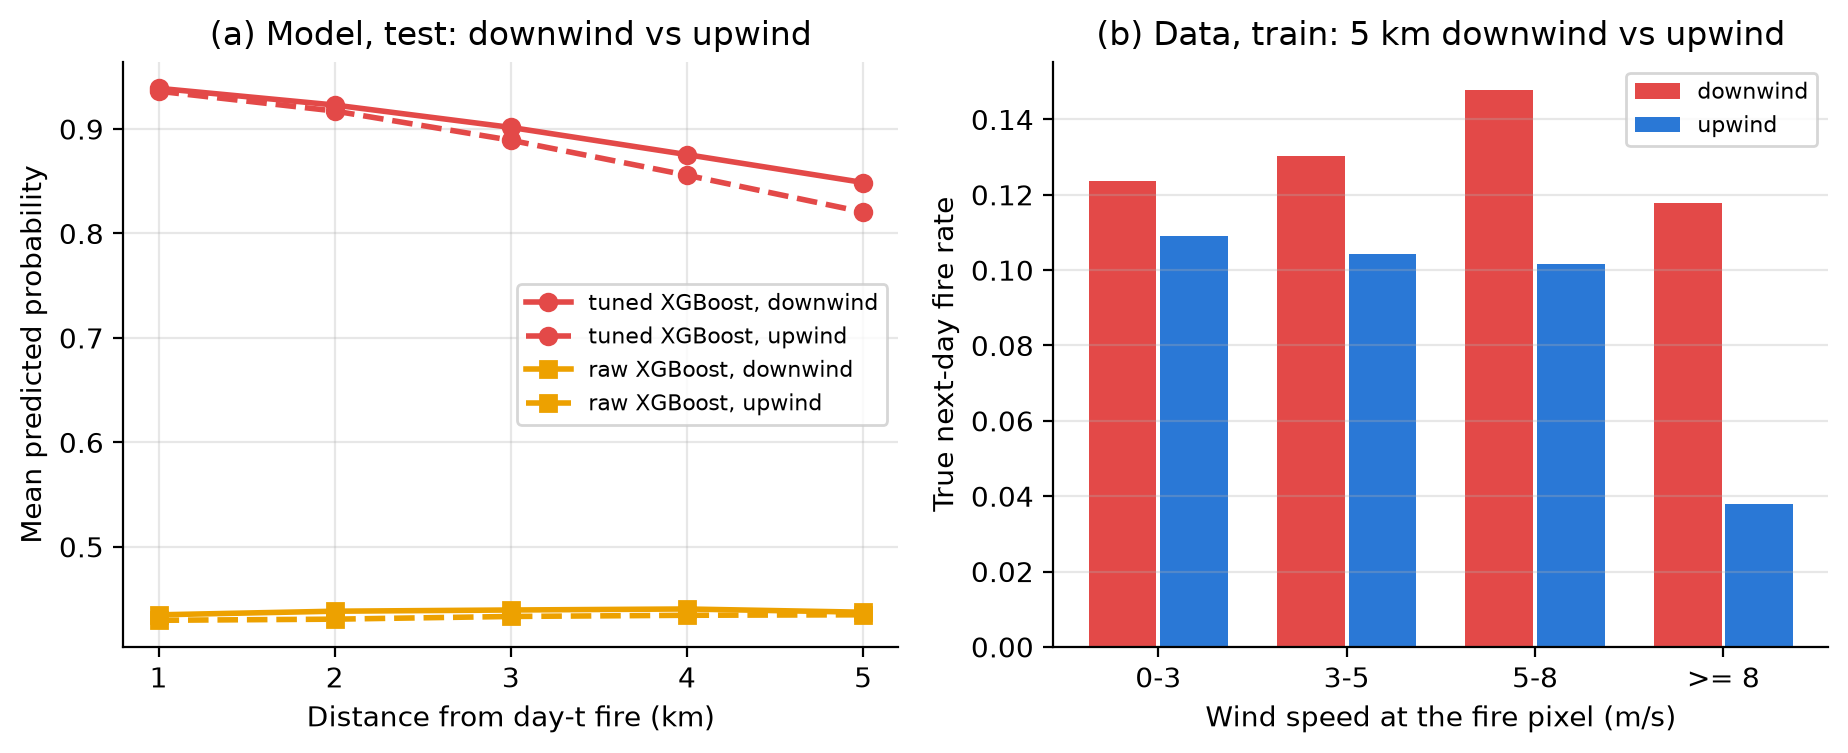
\includegraphics[width=\columnwidth]{figures/eval_downwind_check.png}
\caption{Downwind check. (a) Mean predicted probability 1--5\,km downwind (solid) and upwind (dashed) of day-$t$ fire,
test split. (b) True next-day fire rate 5\,km downwind and upwind of day-$t$ fire by wind speed, train split.}
\label{fig:wind}
\end{figure}

To test whether the model pushes risk downwind, we step 1--5 pixels downwind and upwind from every day-$t$ fire pixel
and compare predictions in pixels not yet burning (Fig.~\ref{fig:wind}a). The tuned model's downwind probability is
higher at every distance, with the gap growing from 0.003 at 1\,km to 0.029 at 5\,km. The training data agrees
(Fig.~\ref{fig:wind}b): 5\,km from the fire, the downwind-to-upwind ratio of next-day fire grows with wind speed, from
1.135 in calm wind (0--3\,m/s) to 3.100 at 8\,m/s or more. Our first version of this check assumed north-up patches and
found the opposite in strong wind, which revealed that the arrays are stored south-up. On test the excess holds only in
calm wind (1.081, against 0.782 and 0.444 at 3--8\,m/s), but these ratios rest on a few large fires
(Section~\ref{sec:events}), so the train split is the more reliable estimate.

\subsection{Error analysis}

\begin{figure}[t]
\centering
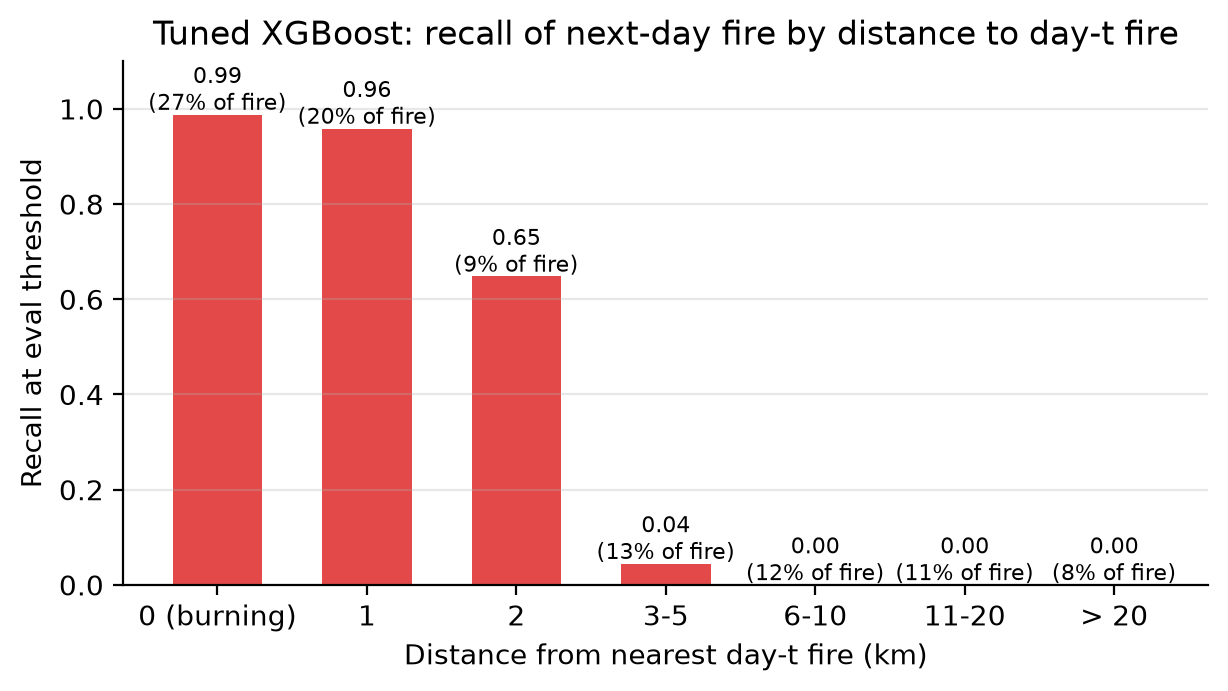
\includegraphics[width=\columnwidth]{figures/eval_recall_by_distance.png}
\caption{Recall of next-day fire pixels by distance to the nearest day-$t$ fire (tuned XGBoost, eval threshold).
Labels give the share of all next-day fire in each band.}
\label{fig:dist}
\end{figure}

At the eval threshold the tuned XGBoost makes 44\,409 true positives, 138\,714 false positives and 39\,922 false
negatives. \textbf{False positives} form a halo around dying fires: 88.8\% lie within 2\,km of day-$t$ fire, and 53.1\%
come from patches whose fire shrinks, although only 38.4\% of test patches shrink; only 35.3\% of day-$t$ fire pixels still
burn on day $t+1$. The five worst patches all hold large, scattered fires (255--468 burning pixels) that shrink the next
day. Nothing in the inputs says which fires will die down (no burnt-out fuel, containment or next-day weather).
\textbf{False negatives} come from long-range spread and sudden growth. Recall falls sharply with distance from the
day-$t$ fire (Fig.~\ref{fig:dist}): 0.988 for burning pixels, 0.959 at 1\,km, 0.648 at 2\,km, 0.044 at 3--5\,km and zero
beyond 5\,km, where 64.4\% of all missed pixels lie. In one patch a fire grows from 8 to 260 pixels in a day and the
halo covers only its centre.

\subsection{Event-level evaluation}
\label{sec:events}

The test split contains duplicate patches and overlapping crops of the same fire, so pooled pixels over-weight large
fires. As the dataset has no fire identifier, we link two test patches when a $16\times16$ elevation block of one
appears exactly inside the other, and treat linked patches as one event. The 1\,689 patches form only 257 events; the 10
largest hold 57\% of next-day fire pixels. Scored per event (240 events with both classes), the tuned XGBoost reaches a
mean PR AUC of 0.187 and a median of 0.120, and the baselines 0.074--0.101, so the ranking holds. At the eval threshold,
however, it finds fire in only 47.9\% of events against 60.8\% for persistence: a threshold that maximises pooled F1 is
driven by the large fires.

\subsection{Limitations and motivation for Phase~2}
A per-pixel model with neighbourhood summaries learns a halo of roughly fixed radius around the day-$t$ fire. It has no
notion of the shape of the fire front, it cannot predict spread beyond a few kilometres, and it cannot tell a growing
fire from a dying one; these are exactly its errors. The hand-made wind features carry real but small signal.
Phase~2 therefore moves to a CNN / U-Net that sees the whole patch, including the fire front and the wind field,
as spatial input.
